\documentclass[a4]{article}

\usepackage[icelandic]{babel}
\usepackage[T1]{fontenc}
\usepackage{amsmath}
\usepackage{graphicx}
\usepackage{sidecap}
\usepackage[utf8]{inputenc}
\usepackage[left=1in,top=1in,right=1in,bottom=1in,nohead]{geometry}
\usepackage[framed,numbered,autolinebreaks,useliterate]{mcode}
\usepackage{amsfonts}
\usepackage{epstopdf}

\title{Töluleg Greining\\ Heimaverkefni 2}
\date{\today{}}
\author{ 
  Bjarki Geir Benediktsson,\and
  Haukur Óskar Þorgeirsson,\and
  Matthías Páll Gissurarson \and
  Kennari: Máni Maríus Viðarsson
  }



\begin{document}
\begin{flushright}
  Bjarki Geir Benediktsson,\\
  Haukur Óskar Þorgeirsson,\\
  Matthías Páll Gissurarson\\
\end{flushright}

\begin{center}
 \textsc{ \LARGE Töluleg Greining\\
  Heimaverkefni 2\\
  \today{}
  }
  \end{center}
\vfill

\maketitle
\section*{Inngangur}
%Bæta við texta
%%%%%%%%%%%%%%
%%%%%%%%%%%%%%
%%%%%%%%%%%%%%
%%%%%%%%%%%%%%
%%%%%%%%%%%%%%
%%%%%%%%%%%%%%
\section*{Feristeikning með splæsibrúun}
\subsection*{Teikning á lokuðum ferlum með aflestri af skjá}
\lstinputlisting{splaesiSkja_1.m}
%Bæta við mynd af keyrslu


\subsubsection{Teikning á þvinguðum ferlum með aflestri af skjá }
\lstinputlisting{splaesiSkja_2.m}
%Bæta við mynd af keyrslu

\subsection{Ferilteikning með Bezier-splæsibrúun}
\lstinputlisting{bezier_bruun.m}
\lstinputlisting{baz.m}
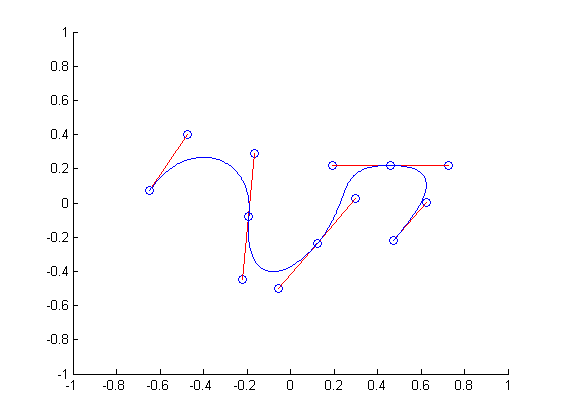
\includegraphics{Einsogpdf.png}
%Hér á að hafa inni fullt af myndarunki


\vspace{20 mm}
Að skýrsluni unnu :
\hspace{0.5cm} \makebox[1.5in]{\hrulefill}
\hspace{0.5cm} \makebox[1.5in]{\hrulefill}
\hspace{0.5cm} \makebox[1.5in]{\hrulefill}
\end{document}
